\subsection{Modulo Network}

El módulo \textit{Network} es el encargado de instanciar todos los elementos ferroviarios presentes en la red de grafos generada por el RNA e interconectarlos como ésta indica. Es el módulo que mas recursos de la FPGA utiliza y donde más se hace énfasis en el uso óptimo de los recursos. Se prioriza la máxima descentralización posible de los módulos instanciados internamente, de forma tal que cada uno de ellos solo dependa de la mínima cantidad necesaria de módulos, evitando conexiones innecesarias. El diagrama de bloques de las máquinas de estado finitas con camino de datos diseñado para lograr este objectivo se muestra en la Figura \ref{fig:Network_module}.

\begin{figure}[H]
	\centering
	\includegraphics[width=1\textwidth]{Figuras/Network_module.png}
	\centering\caption{FSMD del módulo \textit{Network}.}
	\label{fig:Network_module}
\end{figure}

Los módulos de \textit{NetElements}, \textit{Routes} y \textit{Signals} son obligatorios ya que se encuentran presentes en la mínima red ferroviaria aceptada por el RNA. En cambio, los módulos de \textit{SingleSwitches}, \textit{DoubleSwitches}, \textit{ScissorCrossings} y \textit{LevelCrossings} son opcionales y dependen de que existan en la locación. Es decir, si un elemento ferroviario no existe, no solamente no serán instanciado por el ACG, sino que tampoco se generarán archivos que definan sus módulos, señales auxiliares que los interconecten a otros módulos ni tampoco entradas o salidas en otros módulos, destinados a este elemento. De esta manera, se reduce la complejidad del sistema enormemente al implementar solamente los puertos, señales, módulos y conexiones que serán utilizados por el sistema de enclavamiento.

Para garantizar la descentralización de la red, a todos los elementos ferroviarios con entidad física, es decir, todos los mencionados menos las rutas que son entidades abstractas, se les implementa la propiedad de enclavamiento. El enclavamiento de un elemento puede presentar tres estados, tal como se describe en la Tabla \ref{Tab:interlock_states}.

	\begin{table}[!h]
	{
		\caption{Estados de enclavamiento de cada elemento ferroviario.}
		\label{Tab:interlock_states}
		\centering
		\resizebox{1\textwidth}{!}{
		\begin{tabular}{ p{5cm} p{4cm} p{4cm} }
			\hline	
			Liberado & Reservado & Enclavado \\	
			\hline
			Solicitado por cualquier ruta u opera de forma automática.& 
			Operado solamente por la ruta que lo reservó.&
			Depende de sí mismo y de la ruta que lo enclavó.\\
			\hline
		\end{tabular}
		}
	}
	\end{table}

Todo elemento se encuentra por defecto en el estado liberado y puede ser solicitado por cualquier ruta. Tan pronto una ruta envía el comando de reserva al elemento, pasa a estar en estado reservado y ninguna otra ruta podrá hacer uso de este elemento. Finalmente, si la ruta ha podido reservar todos los elementos necesarios para cumplir las condiciones para ser habilitada, enviará la señal de enclavamiento a todos los elementos involucrados, evitando que puedan ser comandados por otras rutas. Esto incluye tanto a la ocupación de vías (\textit{NetElements}) como a las señales (\textit{Signals}), pasando por todos los cambios de vías (\textit{SingleSwitches}, \textit{DoubleSwitches} y \textit{ScissorCrossings}) y barreras de pasos a nivel (\textit{LevelCrossings}). De esta manera el ACG se asegura que cada elemento sea controlado por una única ruta por vez o de forma automática si ninguna ruta demanda su uso.

A diferencia de los módulos explicados en secciones anteriores, donde cada módulo era instanciado una vez, los módulos que modelan elementos ferroviarios, con entidad física o abstracta, son instanciados tantas veces como unidades de éstos existan. Es por eso que, en las siguientes secciones, hablaremos de módulos genéricos a la hora de describir cada módulo. Estos módulos genéricos presentarán todas las entradas, salidas y funcionalidades que pueden tener, de ser requeridas. 

Es trabajo del ACG determinar cuales de ellas deben ser implementadas y cuales no. Por ejemplo, si una ruta A requiere que una barrera X se encuentre baja, pero no tiene requerimientos respecto a las posiciones de los cambios porque la ruta A no los utiliza, entonces el ACG instanciará el módulo de la ruta A considerando en las entradas y salidas los estados de la barrera X y los comandos para operarla, intercontando el módulo de ruta A con el módulo de la barrera ferroviaria X. En cambio, el ACG no implementará ningún puerto destinado a los cambios de vías ni lo considerará en las funcionalidades del módulo de ruta A. De igual manera, el ACG conectará los estados de ocupación de vías correspondientes solamente a los módulos de los elementos ferroviarios que los necesitan y no la totalidad del vector de datos.

\subsection{Módulo genérico de las barreras ferroviarias}

\lipsum[1]

\begin{figure}[H]
	\centering
	\includegraphics[width=1\textwidth]{Figuras/LCB_module}
	\centering\caption{FSMD del módulo genérico de \textit{LevelCrossing}.}
	\label{fig:LCB_module}
\end{figure}

\lipsum[1]

\begin{figure}[H]
	\centering
	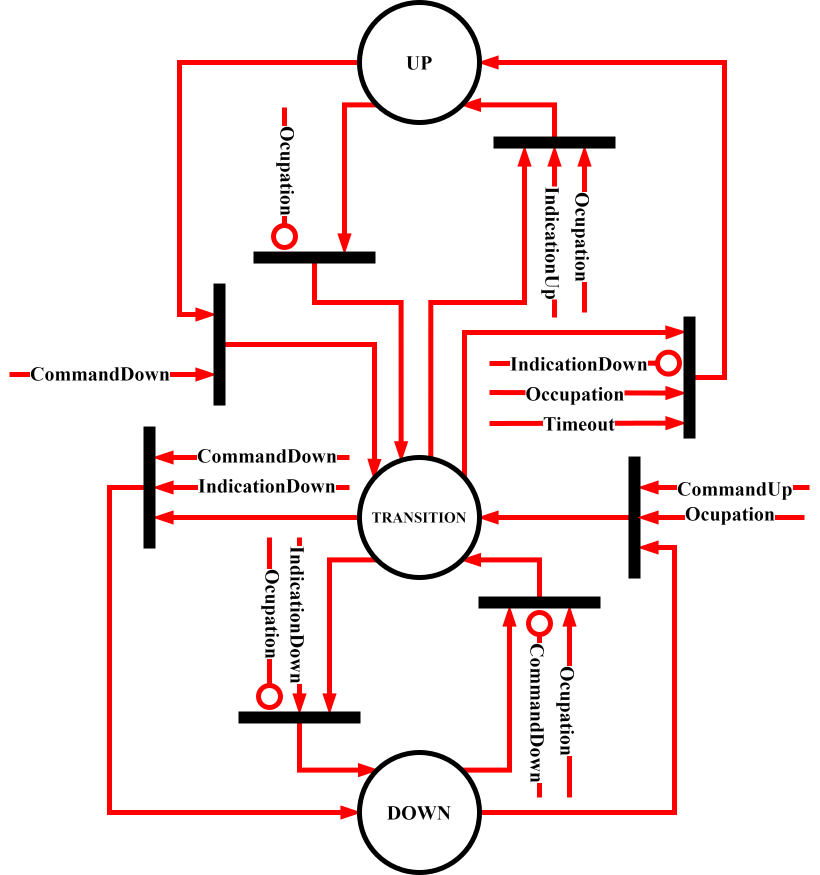
\includegraphics[width=1\textwidth]{Figuras/LCB_petri}
	\centering\caption{Red de petri del modelo dinámico de \textit{LevelCrossing}.}
	\label{fig:LCB_module}
\end{figure}

\lipsum[1]
\subsection{Módulo genérico de los cambios de vías simples}

\lipsum[1]

\begin{figure}[H]
	\centering
	\includegraphics[width=1\textwidth]{Figuras/SSW_module}
	\centering\caption{FSMD del módulo genérico de \textit{SingleSwitches}.}
	\label{fig:SSW_module}
\end{figure}

\lipsum[1]

\begin{figure}[H]
	\centering
	\includegraphics[width=1\textwidth]{Figuras/SSW_Petri}
	\centering\caption{Red de Petri del modelo dinámico de \textit{SingleSwitches}.}
	\label{fig:SSW_Petri}
\end{figure}

\lipsum[1]

\subsection{Módulo genérico de los cambios de vías dobles}

\lipsum[1]

\begin{figure}[H]
	\centering
	\includegraphics[width=1\textwidth]{Figuras/DSW_module}
	\centering\caption{FSMD del módulo genérico de \textit{DoubleSwitches}.}
	\label{fig:DSW_module}
\end{figure}

\lipsum[1]
\subsection{Módulo genérico de los cambios en tijeras}
	\label{sec:ACG_scr}
		
	El módulo \textit{ScissorCrossings} es el encargado de implementar el funcionamiento de los cambios de vías en tijeras en la red ferroviaria. Su implementación es similar a la del módulo \textit{SingleSwitches}, con el ACG utilizando la información otorgada por el RNA para implementar las entradas y salidas necesarias para habilitar el movimiento del cambio de vías solo en situaciones seguras y confirmando su correspondencia mediante la comparación del comando y la indicación. El diagrama de bloques de las máquinas de estado finitas con camino de datos diseñado para lograr este objetivo se muestra en la Figura \ref{fig:SCR_module}.
	
	\begin{figure}[H]
		\centering
		\includegraphics[width=1\textwidth]{Figuras/SCR_module}
		\centering\caption{FSMD del módulo genérico de \textit{ScissorCrossings}.}
		\label{fig:SCR_module}
	\end{figure}
	
	Tal se explicó en la Sección \textit{SingleSwitches}, los cambios de vías en tijeras tienen dos posiciones estables: normal y reversa. A diferencia de los cambios de vías simples, donde la posición normal es la posición de mayor prioridad, ya que permite la circulación por vía principal; los posiciones en los cambios de vías en tijeras tienen igual prioridad, ya que ambas posiciones permiten la circulación por vías de igual categoría, pudiendo ser ambas principales. Por lo tanto, aun cuando por defecto se mantiene la funcionalidad de que un cambio de vías retorne a su posición original luego de llegar al timeout sin poder concretar el movimiento, esta función puede desactivarse y dejar el cambio en una posición intermedia luego de un timeout. El comportamiento de los cambios de vías dobles es mucho más complejo, tal como se define en la red de Petri de la Figura \ref{fig:DSW_Petri}.
	
	\begin{figure}[H]
		\centering
		\includegraphics[width=1\textwidth]{Figuras/SSW_Petri}
		\centering\caption{Red de Petri del modelo dinámico de \textit{ScissorCrossings}.}
		\label{fig:SCR_Petri}
	\end{figure}
	
	En definitiva, los cambios de vías presentan diferencias en sus modelos dinámicos de comportamiento y en el tamaño de los puertos de comando, indicación y correspondecia, pero a grandes rasgos presentan muchas similitudes que son aprovechadas por el ACG. Entre las ventajas encontradas tenemos el uso de una plantilla común a la hora de definir los módulos y sus máquinas de estados, agilizando el proceso de desarrollo del ACG. Además, ésto facilita la comprobación y validación de los módulos al compartir raíces comunes.

\subsection{Módulo genérico de los netElements}

\lipsum[1]

\begin{figure}[H]
	\centering
	\includegraphics[width=1\textwidth]{Figuras/NET_module}
	\centering\caption{FSMD del módulo genérico de \textit{NetElements}.}
	\label{fig:NET_module}
\end{figure}

\lipsum[1]

\begin{figure}[H]
	\centering
	\includegraphics[width=1\textwidth]{Figuras/NET_Petri}
	\centering\caption{Red de Petri del modelo dinámico de \textit{NetElements}.}
	\label{fig:NET_Petri}
\end{figure}

\lipsum[1]

\subsection{Modelo dinámico de las señales ferroviarias}

\lipsum[1]

\begin{figure}[H]
	\centering
	\includegraphics[width=1\textwidth]{example-image}
	\centering\caption{xxxxx}
	\label{fig:XXXX}
\end{figure}

\lipsum[1]
\subsection{Módulo genérico de las rutas ferroviarias}

\lipsum[1]

\begin{figure}[H]
	\centering
	\includegraphics[width=1\textwidth]{Figuras/RTS_module}
	\centering\caption{FSMD del módulo genérico de \textit{Routes}}
	\label{fig:RTS_module}
\end{figure}

\lipsum[1]